\documentclass{article}

\usepackage{enumitem}
\usepackage{mathtools}
\usepackage{amsthm}
\usepackage[noend]{algpseudocode}

\title{Answers to CSCI 570 - Fall 2021 - HW 5}
\author{Shangning Xu}

\begin{document}

\maketitle

\begin{enumerate}
    \item   
    \begin{enumerate}[label=\alph*)]
        \item $\Theta(n^2\log^2 n)$. We have
        \begin{align*}
            T(n) &= \Theta(n^2) + \sum_{j = 0}^{\log_2 n - 1} 4^j\left(\frac{n}{2^j}\right)^2 \log\frac{n}{2^j}\\
            &= \Theta(n^2) + \sum_{j = 0}^{\log_2 n - 1} n^2 (\log n - j\log 2)\\
            &= \Theta(n^2) + n^2(\log n\log_2 n - \frac{\log 2}{2}\log_2 n(\log_2 n - 1))\\
            &= \Theta(n^2\log^2 n)
        \end{align*}
        \item The first case of the master theorem applies here, giving $\Theta(n^{\log_6 8})$.
        \item Case 3 of the master theorem applies here, giving $\Theta(n^{\sqrt{6000}})$.
        \item Case 3 of the master theorem applies here, giving $\Theta(2^n)$.
        \item Renaming $m = \log_2 n$ yields
        \[
            T(2^m) = 2T(2^{m/2}) + m.
        \]
        We can now rename $S(m) = T(2^m)$ to produce a new recurrence
        \[
            S(m) = 2T(m/2) + m,
        \]
        which has a solution of $S(m) = \Theta(m\log m)$. Changing back from $S(m)$ to $T(n)$, we obtain
        \[
            T(n) = T(2^m) = S(m) = \Theta(\log n\log\log n).
        \]
    \end{enumerate}

    \item
    \begin{enumerate}
        \item
        \begin{proof}
            Suppose that $A$ doesn't have any local minimum. Then, for $1 < i < n$, either $A[i] > A[i - 1]$ or $A[i] > A[i + 1]$. Now, we will prove $A[i - 1] \ge A[i]$ for $1 < i < n$ by induction.

            \begin{enumerate}
                \item The base case when $i = 2$ is trivial, as we already have $A[1] \ge A[2]$.
                \item Now assume that $A[k - 1] \ge A[k]$. For $i = k + 1 < n$, it must be the case that $A[k + 1] > A[k + 2]$ as there must not be any local minimum.
            \end{enumerate}

            The induction above gives $A[n - 2] \ge A[n - 1]$ for $i = n - 1$, which, along with $A[n - 1] \le A[n]$, shows that there really is a local minimum at index $n - 1$, contradicting our assumption.
        \end{proof}
        \item To find a local minium, we start with the entire array, find its midpoint $m$ and choose the left half if $A[m] \le A[m + 1]$ (otherwise the right half), until the range converges to one element, which is a local minimum. Because we only choose half the range each time, the number of comparison operations can be described as $T(n) = T(n/2) + 1$, giving a complexity of $\Theta(\log n)$.
    \end{enumerate}

    \item Case 1 of the master theorem applies to ALG's recurrence, giving $T(n) = \Theta(n^{\log_2 7})$. For $T'(n)$, case 1 of the master theorem applies only when $a > 16$ because $n^2\log n = O(n^{\log_4 a - \epsilon})$ for $0 < \epsilon < \log_4 a - 2$, giving $T'(n) = \Theta(n^{\log_4 a})$. As ALG' is not asymptotically slower than ALG, we have $\log_4 a \le \log_2 7$. Solving for $a$ gives $a \le 49$, with a maximum value of 49.
    
    \item Given a collection of cards of size $n$, we will divide them into two piles $p_1$ and $p_2$ and apply our procedure recursively to each pile to find the group of equivalent cards whose size is more than half the pile size. We can at most find two such groups $G_1$ and $G_2$ of cards, each for one pile.

    Now we show how to find the group of equivalent cards whose size is more than $n/2$ in the original collection. If such group $G$ exists, no matter how the collection is divided into two piles, at least one pile will have more than $n/4$ cards from $G$. That is, either $G_1$ or $G_2$ must be equivalent to $G$. Therefore, we only need to pick a card from $G_1$, test its equivalency with all cards in $p_2$, and vice versa for $G_2$ and $p_1$. After testing, the one among $G_1$ and $G_2$ whose size increases to more than $n/2$ must be the group $G$.

    \item We present the following algorithm:
    \begin{algorithmic}[1]
        \State $r \gets T.root$
        \State Let $a$ be the node with smaller value between $x$ and $y$ and $b$ be the greater.
        \While{true}
            \If{$r.value > b.value$}
                \State $r \gets r.left$
            \ElsIf{$r.value < a.value$}
                \State $r \gets r.right$
            \Else
                \State \Return $r$
            \EndIf
        \EndWhile
    \end{algorithmic}

    Because during each iteration, we either return the result or choose a subtree, effectively halving the problem size, the algorithm is described by the recurrence $T(n) = T(n/2) + c$. Solving the recurrence gives a runtime of $T(n) = \Theta(\log n)$.

    \item
    \begin{enumerate}[label=\alph*)]
        \item We present the following algorithm\footnote{The algorithm given in the reference solution is wrong. Before grading, please test the merge algorithm used for grading with Figure~\ref{fig:6a}.} to merge to skylines. The algorithm may continue into the next page.

        \begin{figure}[bt]
            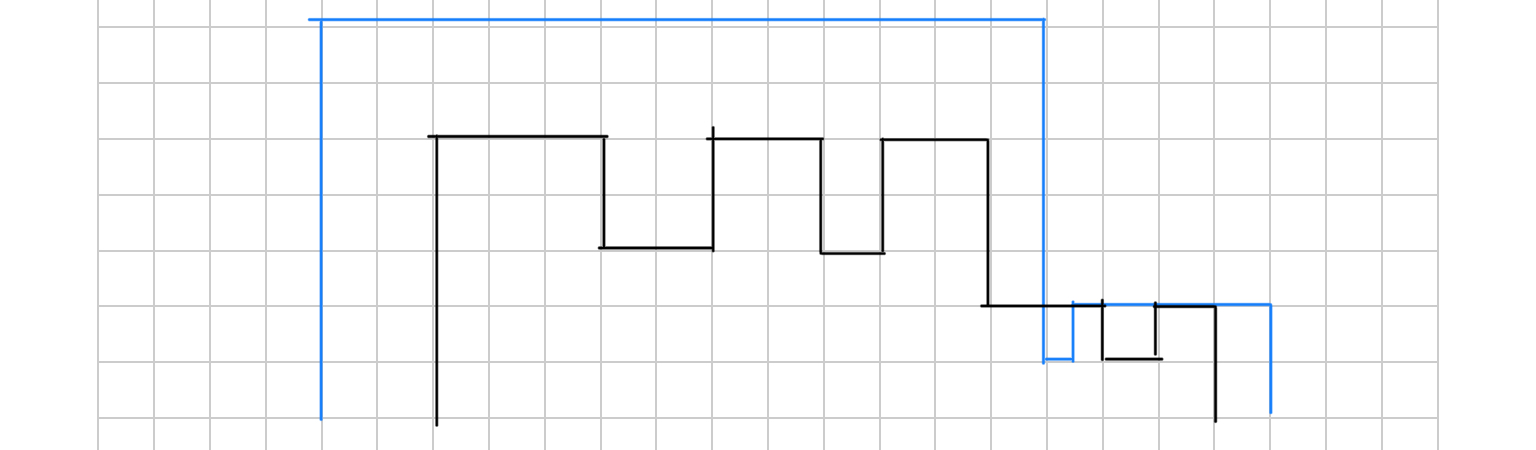
\includegraphics[width=\linewidth]{img/5-6a-example.jpeg}
            \caption{The example for 6 a)}
            \label{fig:6a}
        \end{figure}
        
        \begin{algorithmic}[1]
            \State Let $(w_1, g_1, w_2, g_2, \dots)$ be the combined skyline
            \State Define $x_0$, $x_0'$, $h_{n + 1}$, $h_{m + 1}'$ and $g_0$ to be 0
            \State $i \gets j \gets k \gets 1$
            \Repeat
                \If{$h_i, h_j' < g_{k - 1}$}
                    \If{$h_{i - 1} \ne h_{j - 1}'$} 
                        \State // If we choose a skyline's height for the last iteration,
                        \State // also choose its $x$-coordinate in this iteration.
                        \State $choose\_x \gets (g_{k - 1} = h_{i - 1})$
                    \Else
                        \State // We don't know what we chose last time.
                        \State $choose\_x \gets (x_i > x_j')$
                    \EndIf
                    \If{$choose\_x$}
                        \State $w_k \gets x_i$
                        \State // Find largest $j$ such that $x_j' \le w_k$.
                        \While{$x_{j + 1}' \le w_k$}
                            \State $j \gets j + 1$
                        \EndWhile
                        \If{$h_j' > h_i$ and $x_j' \le w_k \le x_{j + 1}'$}
                            \State $g_k \gets h_j'$
                        \Else
                            \State $g_k \gets h_i$
                        \EndIf
                    \Else
                        \State $w_k \gets x_j'$
                        \While{$x_{i + 1} \le w_k$}
                            \State $i \gets i + 1$
                        \EndWhile
                        \If{$h_i > h_j'$ and $x_i \le w_k \le x_{i + 1}$}
                            \State $g_k \gets h_i$
                        \Else
                            \State $g_k \gets h_j'$
                        \EndIf
                    \EndIf
                    \State $i \gets i + 1$
                    \State $j \gets j + 1$
                \Else
                    \If{$x_i < x_j'$}
                        \State // If equal, the skyline is ``absorbed'' into the current
                        \State // skyline.
                        \If{$h_i \ne g_{k - 1}$}
                            \State $(w_k, g_k) \gets (x_i, h_i)$
                        \EndIf
                        \State $i \gets i + 1$
                    \Else
                        \If{$h_j' \ne g_{k - 1}$}
                            \State $(w_k, g_k) \gets (x_j', h_j')$
                        \EndIf
                        \State $j \gets j + 1$
                    \EndIf
                \EndIf
                \State $k \gets k + 1$
                \State // Directly append one skyline when the other has been
                \State // exhausted.
                \If{$i = n + 1$}
                    \While{$j \le m$}
                        \State $(w_k, g_k) \gets (x_j', h_j')$
                        \State $j \gets j + 1$
                    \EndWhile
                \ElsIf{$j = m + 1$}
                    \While{$i \le n$}
                        \State $(w_k, g_k) \gets (x_i, h_i)$
                        \State $i \gets i + 1$
                    \EndWhile
                \EndIf
            \Until{$g_k = 0$}
            \State \Return $(w_1, g_1, w_2, g_2, \dots, w_k)$
        \end{algorithmic}

        \item To draw the skyline, we will recursively divide the buildings into two sets, draw each set's skyline and combine two skylines using algorithm from (a). The time complexity can be described with the recurrence $T(n) = 2T(n/2) + O(n)$, giving $T(n) = O(n\log_2 n)$
    \end{enumerate}
\end{enumerate}

\end{document}
